\documentclass{article}
\usepackage{graphicx}
\usepackage{listings}
\usepackage{amsmath}
\usepackage{geometry}
\usepackage{xcolor}
\geometry{a4paper, left=0.2in, right=1in, top=1in, bottom=1in}
\definecolor{codegreen}{rgb}{0,0.6,0}
\definecolor{codegray}{rgb}{0.5,0.5,0.5}
\definecolor{codepurple}{rgb}{0.58,0,0.82}
\definecolor{backcolour}{rgb}{0.95,0.95,0.92}

% Define code listing style
\lstdefinestyle{mystyle}{
    backgroundcolor=\color{backcolour},
    commentstyle=\color{codegreen},
    keywordstyle=\color{blue},
    numberstyle=\tiny\color{codegray},
    stringstyle=\color{codepurple},
    basicstyle=\ttfamily\small,
    breakatwhitespace=false,
    breaklines=true,
    captionpos=b,
    keepspaces=true,
    numbers=left,
    numbersep=5pt,
    showspaces=false,
    showstringspaces=false,
    showtabs=false,
    tabsize=2
}

\lstset{style=mystyle}

\begin{document}


\begin{titlepage}
    \centering
    %\vspace*{\fill}
    
\includegraphics[width=0.2\textwidth]{ruet-monogram.png} \par
    \vspace{1cm}
    {\scshape\LARGE RAJSHAHI UNIVERSITY OF ENGINEERING AND TECHNOLOGY \par}
    \vspace{1cm}
    {\scshape\Large Laboratory Reports\par}
    \vspace{1.5cm}
    {\huge\bfseries Numerical Methods Experiments\par}
    \vspace{2cm}
    \textbf{Submitted to:}\par
    \textbf{Shyla Afroge} \par
    Assistant Professor, Department of CSE \par
    Rajshahi University of Engineering And Technology\par
    \vspace{1cm}
    \textbf{Submitted by:}\par
    Md Naim Parvez \par
    Section: A\par
    Roll : 2003015 \par
    Department of CSE \par
    Rajshahi University of Engineering And Technology\par
    
    \vspace*{\fill}
    %{\large \today\par}
\end{titlepage}

\section*{\centering Lab- 1}

\subsection*{Name of the Experiment}
Root Finding Methods - Bisection and False Position

\subsection*{Theoretical Background}

\subsubsection*{Bisection Method}
The Bisection method is based on the Intermediate Value Theorem, which states that if a continuous function $ f(x) $ changes sign over an interval $ [a, b] $, then there exists at least one root in that interval. The algorithm iteratively narrows down the interval by calculating the midpoint $ x_{\text{mid}} $ and checking for a sign change. The process continues until the interval becomes sufficiently small.

Formula:
\[ x_{\text{mid}} = \frac{a + b}{2} \]

\subsubsection*{False Position Method}
The False Position method, also known as the Linear Interpolation method, utilizes linear interpolation between the function values at the interval endpoints. It estimates the root by finding the x-intercept of the linear segment connecting $ (a, f(a)) $ and $ (b, f(b)) $.

Formula:
\[ x = \frac{af(b) - bf(a)}{f(b) - f(a)} \]

\subsection*{Source Code}
\begin{lstlisting}[language=C++]
#include <iostream>
#include <cmath>

using namespace std;

double f(double x) {
    return x * x * x - 2 * x - 5;
}

double false_position(double a, double b, double tol, int max_iterations) {
    double x, error;

    for (int n = 1; n <= max_iterations; ++n) {
        x = (a * f(b) - b * f(a)) / (f(b) - f(a));
        error = fabs(x - a);

        cout << n << "\t" << a << "\t" << b << "\t" << x << "\t" << f(x) << "\t" << error << endl;

        if (error <= tol)
            return x;

        if (f(x) * f(a) < 0)
            b = x;
        else
            a = x;
    }

    return -1.0; // Return -1 to indicate failure to converge
}

int main() {
    double a, b, tol;
    int max_iterations = 1000; // Maximum number of iterations for both methods

    cout << "Enter a: ";
    cin >> a;
    cout << "Enter b: ";
    cin >> b;
    cout << "Enter the tolerance (e.g., 0.0002): ";
    cin >> tol;

    if (f(a) * f(b) >= 0) {
        cout << "The chosen bounds do not have opposite signs.
         Bisection and false position methods may not converge." << endl;
        return 1;
    }

    int choice;
    cout << "Choose a method:" << endl;
    cout << "1. Bisection" << endl;
    cout << "2. False Position" << endl;
    cin >> choice;

    if (choice == 1) {
        cout << "n\t  a\t\t  b\t\t  x\t\t  f(x)\t\t  Error" << endl;
        cout << "--------------------------------------------------------" << endl;

        // Bisection method
        double x_bisection, error_bisection;
        for (int n = 1; n <= max_iterations; ++n) {
            x_bisection = (a + b) / 2.0;
            error_bisection = fabs(b - a) / 2.0;

            cout << n << "\t" << a << "\t" << b << "\t" << x_bisection << "\t" 
            << f(x_bisection) << "\t" << error_bisection << endl;

            if (error_bisection <= tol)
                break;

            if (f(x_bisection) * f(a) < 0)
                b = x_bisection;
            else
                a = x_bisection;
        }

        cout << "--------------------------------------------------------" << endl;
        cout << "Approximate root using bisection: " << x_bisection << endl;
    } else if (choice == 2) {
        cout << "n\t  a\t\t  b\t\t  x\t\t  f(x)\t\t  Error" << endl;
        cout << "--------------------------------------------------------" << endl;

        // False position method
        double x_false_position = false_position(a, b, tol, max_iterations);

        if (x_false_position != -1.0) {
            cout << "Approximate root using false position: " << x_false_position << endl;
        } else {
            cout << "False position method did not converge within
             the maximum number of iterations." << endl;
        }
    } else {
        cout << "Invalid choice." << endl;
    }

    return 0;
}
\end{lstlisting}
\subsection*{Output (Screenshot)}
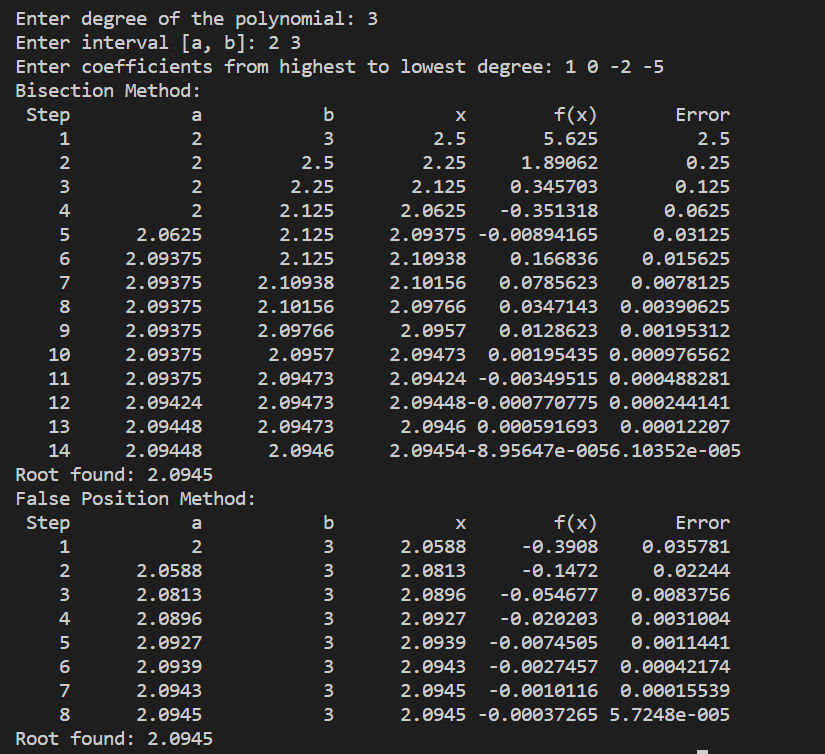
\includegraphics[width=7cm]{lab1.png}
\subsection*{Discussion}
The Bisection method converges slowly but is guaranteed to converge for continuous functions. The False Position method, while potentially faster, may suffer from convergence issues if the chosen interval is not well-behaved. Analyze the impact of the initial interval and tolerance on convergence. Discuss situations where each method excels or struggles.

\clearpage

\section*{\centering Lab- 2}

\subsection*{Name of the Experiment}
Newton's Interpolation Methods - Forward and Backward

\subsection*{Theoretical Background}

\subsubsection*{Newton's Forward Interpolation}
Newton's Forward Interpolation constructs an interpolating polynomial using forward divided differences. The method involves computing the differences of function values at consecutive data points and using them to build up the polynomial.

Formula:
\[ P_n(x) = f(x_0) + (x - x_0) \frac{\Delta f(x_0)}{h} + \frac{(x - x_0)(x - x_1)}{2!} \frac{\Delta^2 f(x_0)}{h^2} + \ldots \]

\subsubsection*{Newton's Backward Interpolation}
Newton's Backward Interpolation, similar to forward interpolation, builds the interpolating polynomial using backward divided differences.

Formula:
\[ P_n(x) = f(x_n) + (x - x_n) \frac{\Delta f(x_n)}{h} + \frac{(x - x_n)(x - x_{n-1})}{2!} \frac{\Delta^2 f(x_n)}{h^2} + \ldots \]

\subsection*{Source Code}
\begin{lstlisting}[language=C++]
#include <iostream>
#include <vector>

using namespace std;

double newtonForwardInterpolation(double x,const vector<double> &xValues,
const vector<double> &yValues)
{
    int n = xValues.size();
    double result = yValues[0];
    double h = xValues[1] - xValues[0];
    double u = (x - xValues[0]) / h;

    vector<vector<double>> dividedDifferences(n, vector<double>(n));

    for (int i = 0; i < n; i++)
    {
        dividedDifferences[i][0] = yValues[i];
    }

    for (int i = 1; i < n; i++)
    {
        for (int j = 0; j < n - i; j++)
        {
            dividedDifferences[j][i] = dividedDifferences[j + 1][i - 1]
             - dividedDifferences[j][i - 1];
        }
    }
    cout<<"Divided Differences Table for Forward method: "<<endl;
    for(int i=0;i<n;i++){
        for(int j=0;j<n;j++){
            cout<<dividedDifferences[i][j]<<" ";
        }
        cout<<endl;
    }

    for (int i = 1; i < n; i++)
    {
        double term = dividedDifferences[0][i];
        for (int j = 0; j < i; j++)
        {
            term *= (u - j) / (j + 1);
        }
        result += term;
    }

    return result;
}

double newtonBackwardInterpolation(double x, const vector<double> &xValues, 
const vector<double> &yValues)
{
    int n = xValues.size();
    double result = yValues[n - 1];
    double h = xValues[1] - xValues[0];
    double u = (x - xValues[n - 1]) / h;

    vector<vector<double>> dividedDifferences(n, vector<double>(n));

    for (int i = 0; i < n; i++)
    {
        dividedDifferences[i][0] = yValues[i];
    }

    for (int i = 1; i < n; i++)
    {
        for (int j = n - 1; j >= i; j--)
        {
            dividedDifferences[j][i] = dividedDifferences[j][i - 1] 
            - dividedDifferences[j - 1][i - 1];
        }
    }
    cout<<"Divided Differences Table for backward method: "<<endl;
    for(int i=0;i<n;i++){
        for(int j=0;j<n;j++){
            cout<<dividedDifferences[i][j]<<" ";
        }
        cout<<endl;
    }

    for (int i = 1; i < n; i++)
    {
        double term = dividedDifferences[n - 1][i];
        for (int j = 0; j < i; j++)
        {
            term *= (u + j) / (j + 1);
        }
        result += term;
    }

    return result;
}

int main()
{
    vector<double> xValues;
    vector<double> yValues;
    double x;

    cout << "Enter the number of data points: ";
    int n;
    cin >> n;

    cout << "Enter the x-values: ";
    for (int i = 0; i < n; i++)
    {
        double value;
        cin >> value;
        xValues.push_back(value);
    }

    cout << "Enter the y-values: ";
    for (int i = 0; i < n; i++)
    {
        double value;
        cin >> value;
        yValues.push_back(value);
    }

    cout << "Enter the value of x: ";
    cin >> x;

    int choice;
    do
    {
        cout << "Menu:" << endl;
        cout << "1. Forward Interpolation" << endl;
        cout << "2. Backward Interpolation" << endl;
        cout << "0. Exit" << endl;
        cout << "Enter your choice: ";
        cin >> choice;
        double backwardInterpolatedValue;
        double forwardInterpolatedValue;
        switch (choice)
        {
        case 1:
            forwardInterpolatedValue = newtonForwardInterpolation(x, xValues, yValues);
            cout << "Forward Interpolated value at x = " << x << " is: "
             << forwardInterpolatedValue << endl;
            break;
        case 2:
             backwardInterpolatedValue = newtonBackwardInterpolation(x, xValues, yValues);
            cout << "Backward Interpolated value at x = " << x << " is: " 
            << backwardInterpolatedValue << endl;
            break;
        case 0:
            cout << "Exiting..." << endl;
            break;
        default:
            cout << "Invalid choice. Please try again." << endl;
            break;
        }
    } while (choice != 0);

    return 0;
}

\end{lstlisting}

\subsection*{Output (Screenshot)}
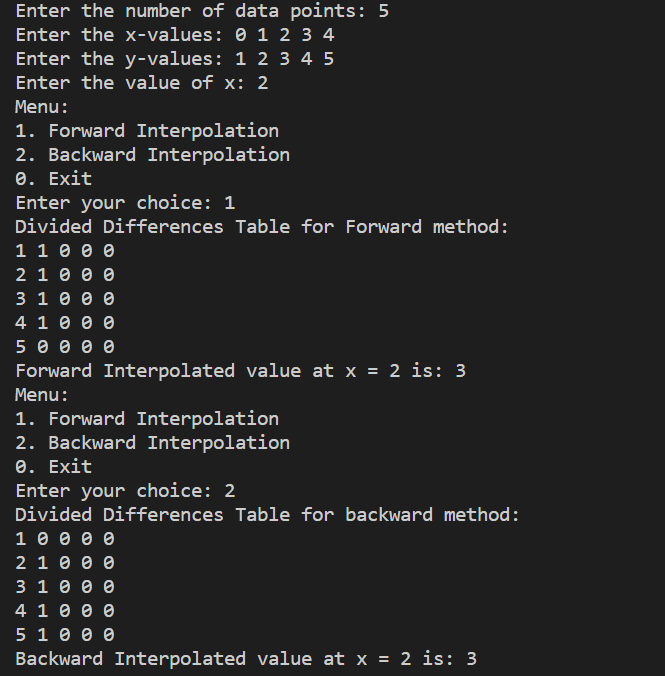
\includegraphics[width=\textwidth]{lab2.png}

\subsection*{Discussion}
Discuss the accuracy of Newton's interpolation methods and their suitability for different datasets. Explore how the number of data points affects the accuracy of interpolation. Consider the computational cost of these methods and any observed oscillations in the interpolated results.

\clearpage

\section*{\centering Lab- 3}

\subsection*{Name of the Experiment}
\textbf{Linear Regression - Data Fitting}

\subsection*{Theoretical Background}
Linear Regression aims to find the best-fitting linear relationship between a set of independent ($x$) and dependent ($y$) variables. The method minimizes the sum of squared differences between the observed and predicted values.

Formula:
\[ y = a + bx \]

where:
\begin{align*}
    a & : \text{Intercept of the linear fit line} \\
    b & : \text{Slope of the linear fit line}
\end{align*}

To find the parameters $a$ and $b$, use the following formulas:

\begin{align*}
    b & = \frac{n(\sum xy) - (\sum x)(\sum y)}{n(\sum x^2) - (\sum x)^2} \\
    a & = \frac{\sum y - b(\sum x)}{n}
\end{align*}

where:
\begin{align*}
    n    & : \text{Number of data points}                             \\
    \sum & : \text{Summation notation}                                \\
    x, y & : \text{Data points (independent and dependent variables)}
\end{align*}

\subsection*{Source Code}
\begin{lstlisting}[language=C++]
#include<bits/stdc++.h>
#include<fstream>
#include<iomanip>
#include<cmath>
#define ll long long
#define fr02m(m) for(int i=0; i<m; i++)
#define fr12m(m) for(int i=1; i<m; i++)
#define fr02j(m) for(int j=0; j<m; j++)
#define frn20(n) for(int i=n; i>=0; i--)
#define frxy(x,y) for(int i=x;i<=y;i++)
#define pb push_back
#define pf push_front
using namespace std;
int main()
{
    int i,j,k,n;
    cout<<"\nEnter the no. of data: \n";       
    cin>>n;
    vector<double>x(n);
    vector<double>y(n);
    double a,b,c;

    cout<<"\nEnter the x-axis values: \n";                
    for (i=0;i<n;i++){
        cin>>x[i];    
    }
    cout<<"\nEnter the y-axis values: \n";
    for (i=0;i<n;i++){
        cin>>y[i];
    }
    double sum_x=0,sum_x2=0,sum_y=0,xysum=0;                
    for (i=0;i<n;i++)
    {
        sum_x=sum_x+x[i];                        
        sum_y=sum_y+y[i];                        
        sum_x2=sum_x2+pow(x[i],2);              
        xysum=xysum+x[i]*y[i];   
    }                 
    a=(n*xysum-sum_x*sum_y)/(n*sum_x2-sum_x*sum_x);           
    c= (sum_y/n) - (a*(sum_x/n));
    cout<<"\nThe linear fit line is of the form:\n\n"<<a<<" + x("<<c<<")"<<endl;        
    return 0;
} 
\end{lstlisting}

\subsection*{Output (Screenshot)}
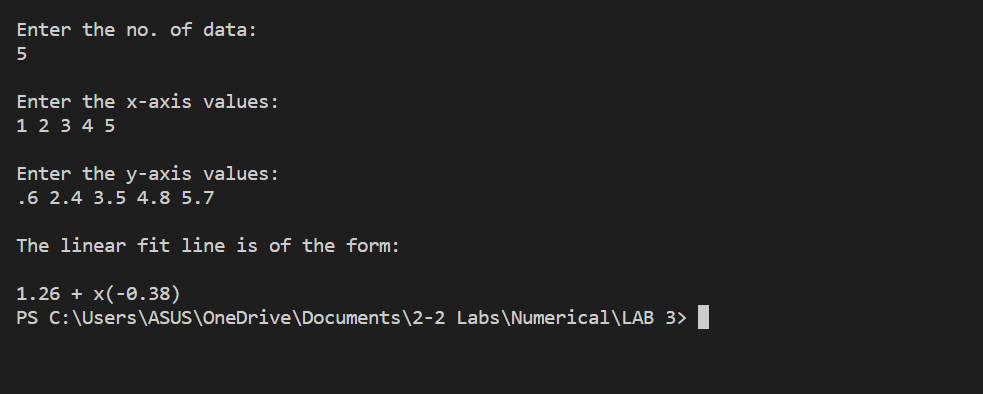
\includegraphics[width=\textwidth]{lab3.png}

\subsection*{Discussion}
Discuss the obtained linear fit line, including the slope ($b$) and intercept ($a$). Examine how well the linear fit represents the given data points. Consider the significance of the linear regression parameters, their interpretation in the context of the specific dataset, and potential limitations of the linear model.

\clearpage

\section*{\centering Lab- 4}

\subsection*{Name of the Experiment}
Numerical Integration Techniques - Trapezoidal, Simpson's 1/3, and 3/8 Rules

\subsection*{Theoretical Background}

\subsubsection*{Trapezoidal Rule}
The Trapezoidal Rule approximates the definite integral by dividing the interval into trapezoids and summing their areas. It is derived from the geometric interpretation of the integral.

Formula:
\[ \int_{a}^{b} f(x) \,dx \approx \frac{h}{2} [f(a) + 2f(x_1) + 2f(x_2) + \ldots + f(b)] \]

\subsubsection*{Simpson's 1/3 Rule}
Simpson's 1/3 Rule uses quadratic interpolating polynomials to approximate the integral. It provides higher accuracy than the Trapezoidal Rule.

Formula:
\[ \int_{a}^{b} f(x) \,dx \approx \frac{h}{3} [f(a) + 4f(x_1) + 2f(x_2) + \ldots + 4f(x_{n-1}) + f(b)] \]

\subsubsection*{Simpson's 3/8 Rule}
Simpson's 3/8 Rule is an extension of Simpson's 1/3 Rule, using cubic interpolating polynomials. It offers further improvement in accuracy.

Formula:
\[ \int_{a}^{b} f(x) \,dx \approx \frac{3h}{8} [f(a) + 3f(x_1) + 3f(x_2) + 2f(x_3) + \ldots + 3f(x_{n-2}) + 3f(x_{n-1}) + f(b)] \]

\subsection*{Source Code}
\begin{lstlisting}[language=C++]
#include <bits/stdc++.h>
#include <fstream>
#define ll long long
#define fr02m(m) for (int i = 0; i < m; i++)
#define fr12m(m) for (int i = 1; i < m; i++)
#define fr02j(m) for (int j = 0; j < m; j++)
#define frn20(n) for (int i = n; i >= 0; i--)
#define frxy(x, y) for (int i = x; i <= y; i++)
#define pb push_back
#define pf push_front
using namespace std;

float calc(float x)
{
    return (1 / (1 + x));
}
float trapezoidal(float a, float b, int n)
{
    float h = (b - a) / n;
    float sum = 0.0;
    cout<<"x      y"<<endl;
    for (int i = 0; i <= n; i++)
    {
        if (i == 0 || i == n)
        {
            sum += calc(a + i * h);
            cout<<a+i*h<<"   "<<calc(a+i*h)<<endl;
        }
        else
        {
            sum += 2 * calc(a + i * h);
            cout<<a+i*h<<"   "<<calc(a+i*h)<<endl;
        }
    }
    return (h / 2) * sum;
}

float simpsons_one_third(float a, float b, int n)
{
    float h = (b - a) / n;
    float sum = 0.0;
    for (int i = 0; i <= n; i++)
    {
        if (i == 0 || i == n)
        {
            sum += calc(a + i * h);
        }
        else if (i % 2 != 0)
        {
            sum += 4 * calc(a + i * h);
        }
        else
        {
            sum += 2 * calc(a + i * h);
        }
    }
    return (h / 3) * sum;
}

float simpsons_three_eight(float a, float b, int n)
{
    float h = (b - a) / n;
    float sum = 0.0;
    for (int i = 0; i <= n; i++)
    {
        if (i == 0 || i == n)
        {
            sum += calc(a + i * h);
        }
        else if (i % 3 == 0)
        {
            sum += 2 * calc(a + i * h);
        }
        else
        {
            sum += 3 * calc(a + i * h);
        }
    }
    return (3 * h / 8) * sum;
}

int main()
{
    float a, b;
    int n;
    cout << "enter upper limit and lower limit: ";
    cin >> b >> a;
    cout << "enter number of sub interval: ";
    cin >> n;
    cout << "Using Trapezoidal Rule intrigation value is : " << trapezoidal(a, b, n)<<"Error- "
    << endl;
    cout<<"Using simpson's one_third Rule intrigation value is :"<<simpsons_one_third(a, b, n)<<"Error- "  << endl;
    cout<<"Using simpson's three_eight Rule intrigation value is:"<<simpsons_three_eight(a, b, n)
    <<"Error- " ;

    return 0;
}

\end{lstlisting}

\subsection*{Output (Screenshot)}
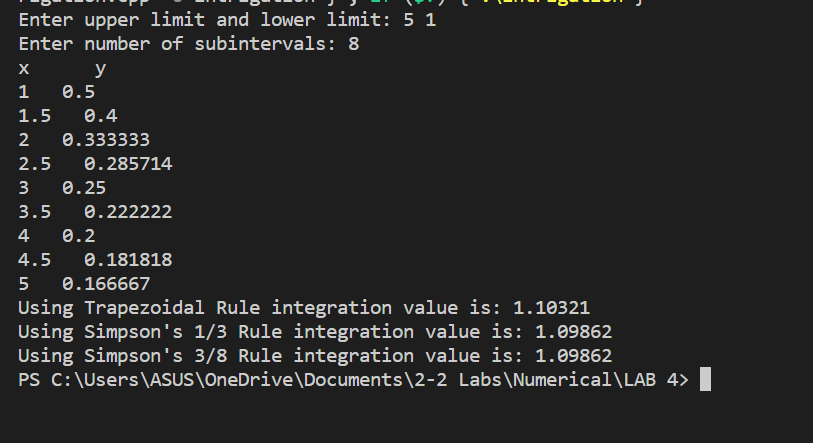
\includegraphics[width=\textwidth]{lab4.png}

\subsection*{Discussion}
Discuss the accuracy and efficiency of each numerical integration method. Analyze the impact of the chosen parameters (number of subintervals) on the results. Compare the results obtained from different integration techniques. Consider the convergence properties and potential sources of error in numerical integration. Discuss situations where each method is most suitable.

\end{document}
